\documentclass[a4paper,10pt]{article}
\usepackage[utf8]{inputenc}
\usepackage{amsmath}
\usepackage{caption}
\usepackage{graphicx}
\usepackage{enumerate}
\title{Lazy Caterer's Sequence}
\author{William Peters, Gihan Mendis}

\begin{document}

\maketitle

\section{Illustration of structures}

\subsection{Pancake Structure}
\begin{enumerate}
  \item $n = 4$\\
  	\begin{enumerate}
    	\item Pancake structure\\
    	\begin{figure}[h!]
			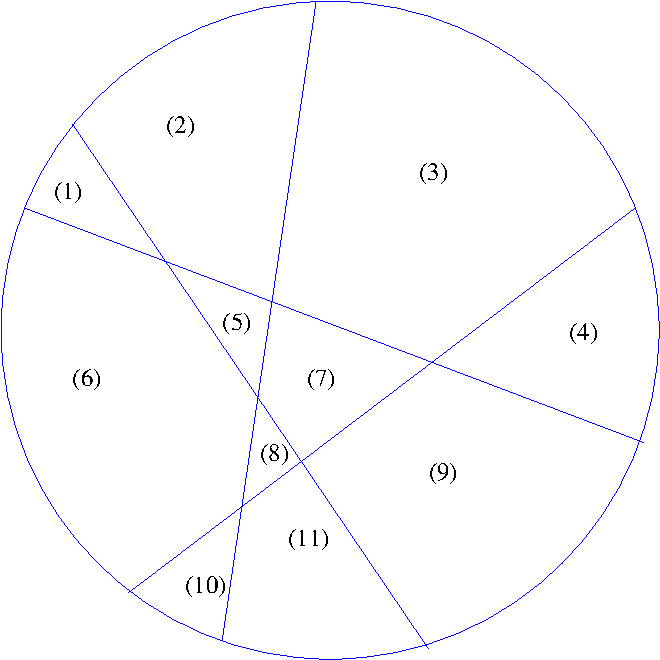
\includegraphics[scale=0.3]{graphics/pancakecut11}
			\captionsetup{labelformat=empty}
			\caption{}
			\label{fig:pancakecut11}
		\end{figure}
  \end{enumerate}
  
  %This should be n = 5 not 4 
  \item $n = 5$\\
  \begin{enumerate}
    \item Pancake structure\\
      \begin{figure}[h!]
			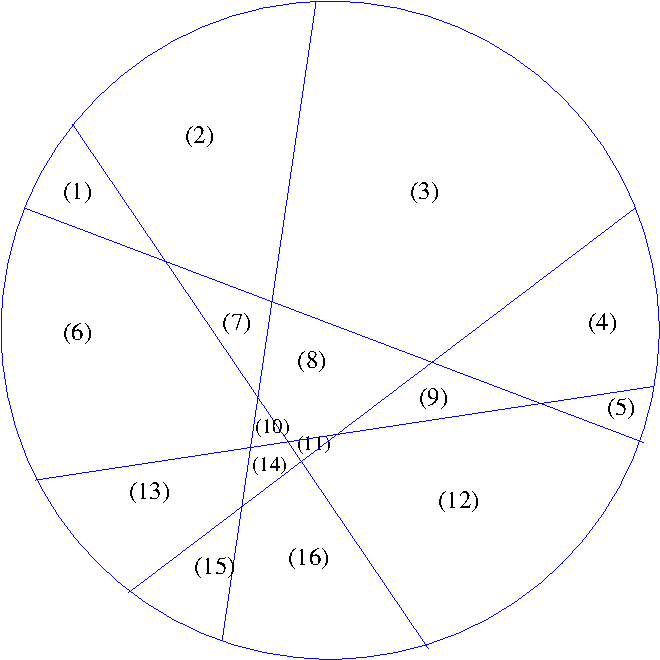
\includegraphics[scale=0.3]{graphics/pancakecut16}
			\captionsetup{labelformat=empty}
			\caption{}
			\label{fig:pancakecut16}
		\end{figure}
  \end{enumerate}
\end{enumerate}

\subsection{Binary Words}
When $n > 3$  the sequence gives the number of binary words where there are at least two ones and at most two two's. In these formulas $n$ represents the length of a binary word, so $a(n)$ gives the number of possible binary words formed with these constraints. The following are two illustrations of this structure. The first is when $n = 4$ and the second is when $n = 5$.

\begin{enumerate}
	\item $n = 4$\\
	\begin{enumerate}
		\item Binary words structure illustration\\
		\[
		\boxed{
		\begin{gathered}
		0011, 0101, 0110, 0111, 1001, 1010, 1011, 1100, 1101, 1110, 1111
		\end{gathered}
		}
		\]
	\end{enumerate}
	
	\item $n = 5$\\
	\begin{enumerate}
		\item Binary words structure illustration\\
		\[
		\boxed{
		\begin{gathered}
		11111, 01111, 10111, 11011, 11101, 11110, 00111, 10011, 10101, 10110,\\ 		        01011, 01101, 01110, 11100, 11001, 11010 
		\end{gathered}
		}
		\]
	\end{enumerate}
\end{enumerate}
 
\section{Formula Demonstrations}
\subsection{Binomial}
\begin{enumerate}
 \item $a(n) = Binomial(n+2,1)-2\times Binomial(n+1,1)+Binomial(n+2,2)$\\

  \hspace{1cm}${n+2 \choose 1} - 2\times {n+1 \choose 1} + {n+2 \choose 2}$\\
  \begin{enumerate}
    \item $n = 4$
    \[
     \boxed{ 
	  \begin{gathered}
       	a(4) = {4+2 \choose 1} - 2\times {4+1 \choose 1} + {4+2 \choose 2}\\
		\\ 
       	a(4) = {6 \choose 1} - 2\times {5 \choose 1} + {6 \choose 2} \\
       	\\
       	a(4) = 6 - 10 + 15\\
       	\\
       	a(4) = 11 
      \end{gathered}	    
	  }
    \]	  
    \item $ n = 5$
    \[
     \boxed{ 
	  \begin{gathered}
       	a(5) = {5+2 \choose 1} - 2\times {5+1 \choose 1} + {5+2 \choose 2}\\
		\\ 
       	a(5) = {7 \choose 1} - 2\times {6 \choose 1} + {7 \choose 2} \\
       	\\
       	a(5) = 7 - 12 + 21\\
       	\\
       	a(4) = 16 
      \end{gathered}	    
	  }
    \]	
  \end{enumerate}
\end{enumerate}

\subsection{Generating Function}
\begin{enumerate}
\item $G.f : A(x) = (1-x+x^2)/(1-x)^3$
  \begin{enumerate}
    \item $n = 4$
    \[
     \boxed{ 
	  \begin{gathered}
    	{[}\frac{d^4 }{dx^4}(1-x+x^2)/(1-x)^3 {]}_{x=0} = 264  \\ 
    	And ~ \frac{264}{4!} = 11 \\
      \end{gathered}	    
	  }
    \]	  
    \item $ n = 5$
    \[
     \boxed{ 
	  \begin{gathered}
		{[}\frac{d^5 }{dx^5}(1-x+x^2)/(1-x)^3 {]}_{x=0} = 1920  \\ 
    	And ~ \frac{1920}{5!} = 16 \\
      \end{gathered}	    
	  }
    \]	
  \end{enumerate}
\end{enumerate}

\subsection{Exponential Generating Function}
\begin{enumerate}
\item $E.g.f: A(x) = e^x+xe^x+\frac{e^xx^2}{2}$
	\begin{enumerate}
		\item $n = 4$
		\[
		\boxed{
			\begin{gathered}
				{[}\frac{d^4}{dx^4}(e^x+xe^x+\frac{e^xx^2}{2}){]}_{x=0} = 11
			\end{gathered}
		}
		\]
		\item $ n = 5$
		\[
		\boxed{
			\begin{gathered}
				{[}\frac{d^5}{dx^5}(e^x+xe^x+\frac{e^xx^2}{2}){]}_{x=0} = 16
			\end{gathered}
		}
		\]
	\end{enumerate}
\end{enumerate}

\subsection{Recursive Formula}
\begin{enumerate}
\item $ a(n+3) = 3*a(n+2)-3*a(n+1) + a(n), a(0) = 1, a(1) = 2, a(2) = 4, a(3) = 7, a(4) = 11, a(5) = 16, a(6) = 22, a(7) = 29, a(8) = 37 $
	\begin{enumerate}
		\item $n = 6$
		\[
		\boxed{
			\begin{gathered}
				a(6+3) = a(9) = 3*a(6+2) - 3*a(6+1) + a(6)\\
				\\
				a(9) = 3*a(8) - 3*a(7) + a(6)\\
				\\
				a(9) = 3*37 - 3*29 + 22\\
				\\
				a(9) = 111-87+22 = 46
			\end{gathered}
			}
		\]
		
		\item $n = 7$
		\[
		\boxed{
			\begin{gathered}
				a(7+3) = a(10) = 3*a(7+2) - 3*a(7+1) + a(7)\\
				\\
				a(10) = 3*a(10) - 3*a(8) + a(7)\\
				\\
				a(10) = 3*46 - 3*37 + 29\\
				\\
				a(10) = 138-111+29 = 56
			\end{gathered}
			}
		\]
		
		\item $n = 8$
		\[
		\boxed{
			\begin{gathered}
				a(8+3) = a(11) = 3*a(8+2) - 3*a(8+1) + a(8)\\
				\\
				a(11) = 3*a(10) - 3*a(9) + a(8)\\
				\\
				a(11) = 3*56 - 3*46 + 37\\
				\\
				a(11) = 168-138+37 = 67
			\end{gathered}
			}
		\]
	\end{enumerate}

\end{enumerate}

\section{Experimental Bijection}

We attempt to define a rule that map maximum set of pancake pieces we can get from n cuts to set of $n$ wordlenght binary words where there are at least two ones and at most two two's. (When  $n > 3$) : \\
\\
We label each pancake cut from "1" to "n" and the original boundary of pancake as "0". Then we consider the boundaries of each piece in alphabetize order as an unique representation of each piece. We attempt to find the bijection of this representation of pancake structure to other binary word structure.\\
\\
Our attempt was illustrated below for when $n=4$.    	    
\\	
\subsection{Demonstration when $n=4$.}
\begin{figure}[h!]
			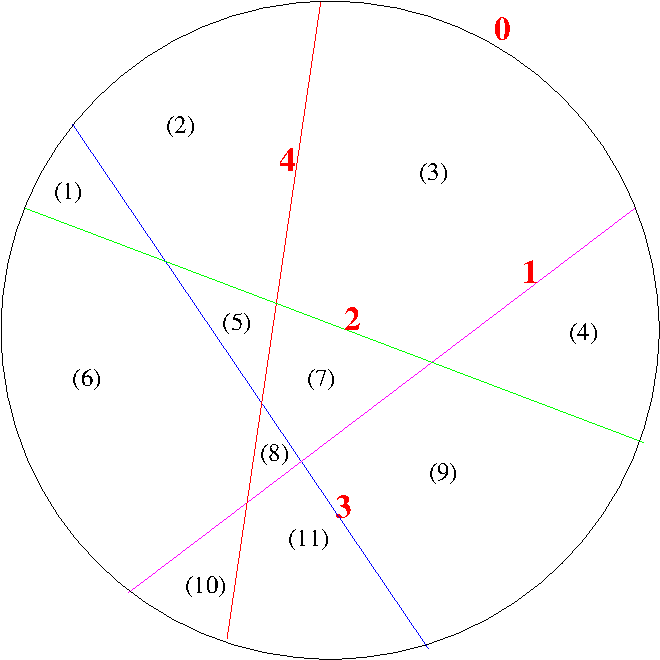
\includegraphics[scale=0.5]{graphics/pancakecut11_bijec}
			\captionsetup{labelformat=empty}
			\caption{}
			\label{fig:pancakecut11}
\end{figure}

By labeling the maximum set of pieces with there boundaries and alphabetize ordering we get the set as follows:\\
\\
${012,0123,01234,0124,0134,014,023,0234,1234,134,234}$ \\
\\
Ordered set of binary number structure is as follows:\\
\\
${0011, 0101, 0110, 0111, 1001, 1010, 1011, 1100, 1101, 1110, 1111}$\\
\\
Bijection we can observe is
%
%Can you write this one I am not really sure what you mean.
%

\section{Experimental Superstructure}

As mentioned in the experimental bijection section the set from the pancake structure can be organize labeling each piece with there boundaries and alphabetize ordering them.Then the superstructure for $n=4$ and $n=5$ are given as bellow. 

\begin{enumerate}
		\item $n=4$\\
		\[
		\boxed{
		\begin{gathered}
	{012,0123,01234,0124,0134,014,023,0234,1234,134,234} \\
		\end{gathered}
		}
		\]
		\item $n=5$\\
		\[
		\boxed{
		\begin{gathered}
		{012,0123,0124,01345,0145,0234,02345,025,034,045,12345,1235,135,145,234,235}
		\end{gathered}
		}
		\]
\end{enumerate}

\end{document}
